\documentclass[compress]{beamer}
\usepackage{graphicx,amsmath,amsthm,verbatim,bm}
\usepackage{longtable}



\usepackage{tabularx}
\usepackage{graphicx}
%\usetheme{Copenhagen}
%\useoutertheme[{options}]{tree}
%\setbeamertemplate{footline}[page number]
%\useoutertheme{infolines}
%\setbeamertem plate{headlirne}{}
\useinnertheme{circles}
\usepackage{comment}
\setbeamertemplate{footline}[frame number]
%\usepackage{times}
%\usepackage[tbtags]{amsmath}
%\usepackage{amssymb}
\usepackage{amsfonts}
%\usepackage{slfortheorems}
\usepackage{epsfig}
\usepackage{graphicx}
\usepackage{tabularx}
\usepackage[small]{caption}
\usepackage[square]{natbib}
%\newcommand{\newblock}{}
\bibpunct{(}{)}{;}{a}{}{,}
\bibliographystyle{ims}
%\usepackage[letterpaper]{geometry}
\usepackage{color}
\setlength{\parindent}{0pt}
\usepackage{bbding}
\usepackage{booktabs} 
\usepackage{xcolor}
\usepackage{lipsum}
\usepackage{algpseudocode}
\usepackage{multirow}
\usepackage{graphicx}
\usepackage{tikz} 
\usetikzlibrary{arrows, snakes, backgrounds, patterns, matrix, shapes, fit, 
calc, shadows, plotmarks}


% Custom commands
\let\oldvec\vec
\let\oldcomment\comment
\renewcommand{\comment}[1]{\textcolor{blue}{[#1]}}
\renewcommand\vec{\bm}
\newcommand{\simfn}{\texttt{sim}} % similarity function
\newcommand{\truncsimfn}{\underline{\simfn}} % truncated similarity function
\newcommand{\partfn}{\texttt{PartFn}} % partition function
\newcommand{\distfn}{\texttt{dist}} % distance function
\newcommand{\valset}{\mathcal{V}} % attribute value set
\newcommand{\entset}{\mathcal{E}} % set of records that make up an entity
\newcommand{\partset}{\mathcal{P}} % set of entities that make up a partition
\newcommand{\1}[1]{\mathbb{I}\!\left[#1\right]} % indicator function
\newcommand{\euler}{\mathrm{e}} % Euler's constant
\newcommand{\eber}{\texttt{EBER}} % Name of Bayesian ER model
\newcommand{\secref}[1]{\S\ref{#1}} % Section reference


\usepackage{listings}
\usepackage[ruled,lined]{algorithm2e}
\def\algorithmautorefname{Algorithm}
\SetKwIF{If}{ElseIf}{Else}{if}{then}{else if}{else}{endif}

\usepackage{longtable}



\theoremstyle{plain}
\usepackage{amsfonts}
\usepackage{epsfig}
\usepackage{graphicx}
%\usepackage[small]{caption}

\usepackage{zref-savepos}

\newcounter{restofframe}
\newsavebox{\restofframebox}
\newlength{\mylowermargin}
\setlength{\mylowermargin}{2pt}

\newenvironment{restofframe}{%
    \par%\centering
    \stepcounter{restofframe}%
    \zsavepos{restofframe-\arabic{restofframe}-begin}%
    \begin{lrbox}{\restofframebox}%
}{%
    \end{lrbox}%
    \setkeys{Gin}{keepaspectratio}%
    \raisebox{\dimexpr-\height+\ht\strutbox\relax}[0pt][0pt]{%
    \resizebox*{!}{\dimexpr\zposy{restofframe-\arabic{restofframe}-begin}sp-\zposy{restofframe-\arabic{restofframe}-end}sp-\mylowermargin\relax}%
        {\usebox{\restofframebox}}%
    }%
    \vskip0pt plus 1filll\relax
    \mbox{\zsavepos{restofframe-\arabic{restofframe}-end}}%
    \par
}


\usepackage{tikz}
\usetikzlibrary{arrows}

%\usepackage[usenames,dvipsnames]{xcolor}
\usepackage{tkz-berge}
\usetikzlibrary{fit,shapes}

\usepackage{calc}
\usetikzlibrary{decorations.markings}

\tikzstyle{vertex}=[circle, draw, inner sep=0pt, minimum size=6pt]
\newcommand{\vertex}{\node[vertex]}
\newcounter{Angle}



%%%to add in new counter for slides in beamer
\newcommand{\beginbackup}{
   \newcounter{framenumbervorappendix}
   \setcounter{framenumbervorappendix}{\value{framenumber}}
}
\newcommand{\backupend}{
   \addtocounter{framenumbervorappendix}{-\value{framenumber}}
   \addtocounter{framenumber}{\value{framenumbervorappendix}} 
}


\newcommand*\oldmacro{}
\let\oldmacro\insertshortauthor
\renewcommand*\insertshortauthor{
  \leftskip=.3cm
\insertframenumber\,/\,\inserttotalframenumber\hfill\oldmacro}




\excludecomment{notbeamer}
\includecomment{beamer}

\newcommand{\lam}{\mathbf{\Lambda}}	
\newcommand{\bX}{\mathbf{X}}
\newcommand{\bY}{\mathbf{Y}}

\title[d-blink: Distributed End-to-End Bayesian Entity Resolution]
{d-blink: Distributed End-to-End Bayesian Entity Resolution}
\author[Rebecca C. Steorts, beka@stat.duke.edu]{Rebecca C. Steorts} 
\institute{\normalsize Department of Statistical Science, affiliated faculty in Computer Science, Biostatistics and Bioinformatics, the information initiative at Duke (iiD) and \\the Social Science Research Institute (SSRI) \\ Duke University and U.S. Census Bureau\\\vspace*{1em}Population Dynamics and Health Program Workshop, University of Michigan }


\date{July 10, 2019}

\begin{document}

\begin{frame}
\titlepage
\end{frame}

\frame{
\frametitle{Motivation} 

\begin{enumerate}
\item Enumerating a census. 
\item Enumerating those that have died in a conflict (such as Syria).
\item Predicting those in poverty in small regions from survey data. 
\item Predicting results of elections from voter registration data. 
\end{enumerate}

Each task may contain duplicated information, which is problematic for the underlying task at hand. 

}


\frame{
\frametitle{Scalable Entity Resolution}
\center
\Large
%\item How does one uniquely estimate entities in real time? 
How does one scale Bayesian entity resolution methods in real time? 


}

\frame{
\frametitle{Entity Resolution}
\center
\Large
Entity resolution (record linkage or de-duplication) is the process of merging together noisy databases to remove duplicate entities. 

%\vspace*{1em}
%
%The downstream task (post-processing task) refers to any inferential or prediction task after entity resolution. 

}

\frame{
\frametitle{The entity resolution graph}
\begin{figure}[htbp]
\begin{center}
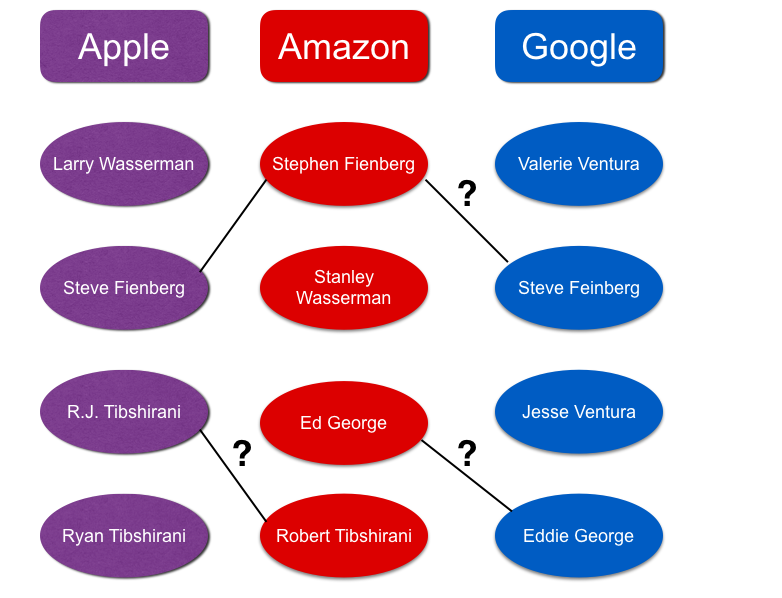
\includegraphics[scale=0.35]{finalFigures/linkage2}
%\caption{default}
%\label{default}
\end{center}
\end{figure}

}

\frame{
\frametitle{The node of Larry Wasserman}
\begin{figure}[htbp]
\begin{center}
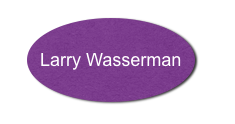
\includegraphics[scale=0.35]{finalFigures/node}
%\caption{default}
%\label{default}
\end{center}
\end{figure}



}

\frame{
\frametitle{The node of Larry Wasserman}
\begin{figure}[htbp]
\begin{center}

\includegraphics[scale=0.35]{finalFigures/node-feature}
%\caption{default}
%\label{default}
\end{center}
\end{figure}



}

\frame{
\frametitle{The entity resolution graph}
\begin{figure}[htbp]
\begin{center}
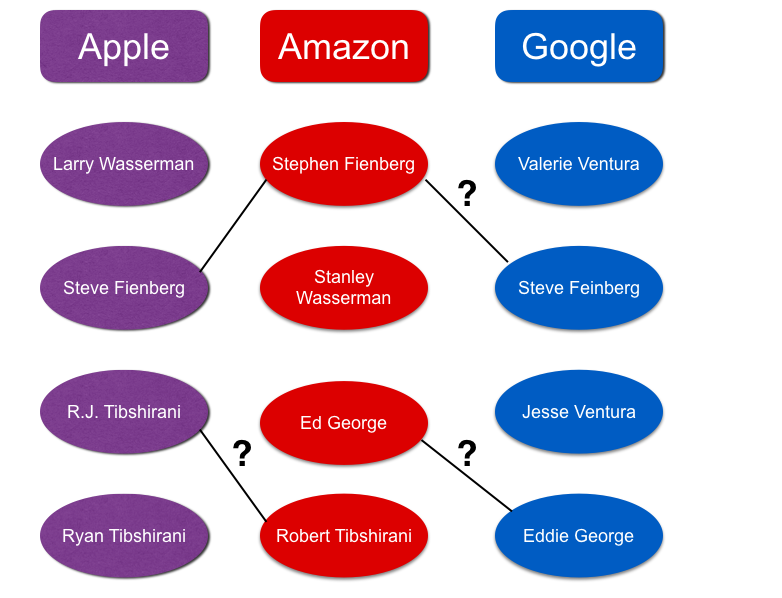
\includegraphics[scale=0.35]{finalFigures/linkage2}
%\caption{default}
%\label{default}
\end{center}
\end{figure}

}

\frame{
\frametitle{Scalable Bayesian entity resolution}
\center
\Large
How does one scale Bayesian entity resolution in real time? 

}

\frame{
\frametitle{Graphical entity resolution}

%\begin{itemize}
%\pause
%\item Dealing with big data means merging large, noisy databases.
%\pause
%\begin{itemize}
%\item Such databases have severe amounts of noise. 
%\end{itemize}
%\pause
%\item Entity resolution requires sophisticated graph structures. [Gutman et. al (2013)].
%\pause
%\begin{itemize}
%\item One approach is to use a bipartite graph for latent entities.
%\pause
%\item Never link records to records. 
%\pause
%\end{itemize}
%\item Computational speed-ups: eliminate low-probability matches.
%%\pause
%%\begin{itemize}
%%\item Blocking techniques based on locality-sensitive hashing.
%\end{itemize}
%\pause

\begin{figure}[htbp]
\begin{center}
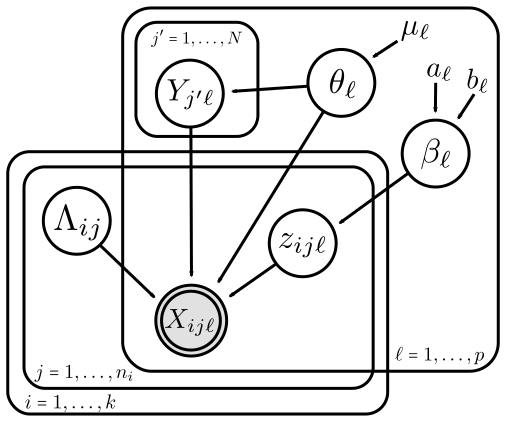
\includegraphics[width=0.6\textwidth]{figures/recordLinkage_graphicalModel}
%\caption{Graphical representation of models \ref{model:cat}-\ref{model:string}.}
\label{fig:graphicalProcess}
\end{center}
\end{figure}


[Copas and Hilton (1990), Tancredi and Liseo (2011), \textbf{RCS}, Hall, Fienberg (2014, 2016); Sadinle (2014, 2016); 
\textbf{RCS} (2015)]. 

}




\frame{

\begin{figure}[htbp]
\begin{center}
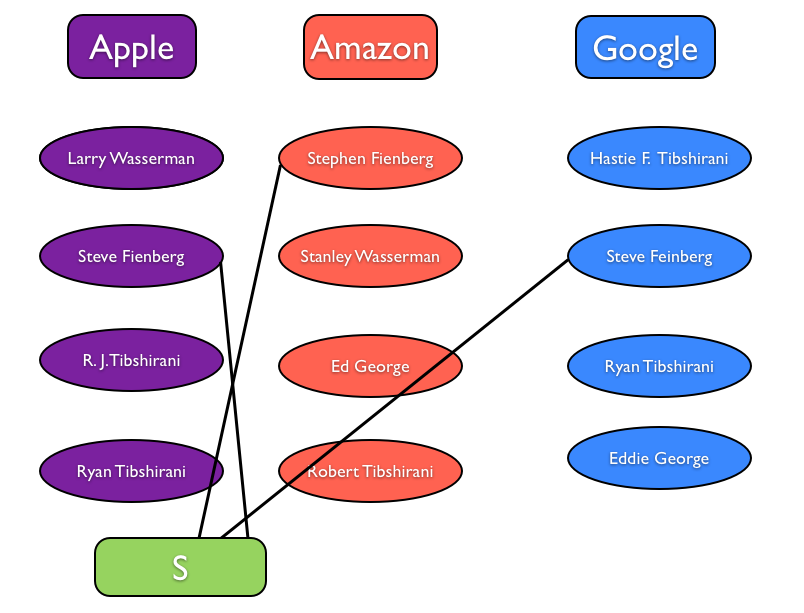
\includegraphics[scale=0.35]{pics/latents_firstex}
%\caption{default}
%\label{default}
\end{center}
%\scriptsize{
%\begin{flushright}
%[Steorts, Hall, and Fienberg (2014), \emph{AIStats}.] \newline
%[Steorts, Hall, and Fienberg (2014), \emph{JASA}, In Revision.], [Steorts (2014), Submitted.] 
%\end{flushright}
%}
\end{figure}

}


\frame{

\begin{figure}[htbp]
\begin{center}
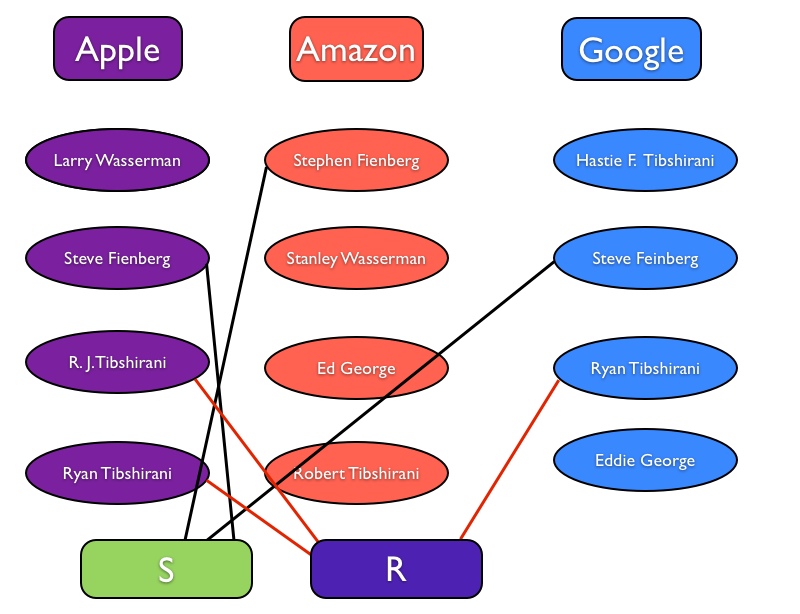
\includegraphics[scale=0.35]{pics/latents_secondex}
%\caption{default}
%\label{default}
\end{center}
%\scriptsize{
%\begin{flushright}
%[Steorts, Hall, and Fienberg (2014), \emph{AIStats}.] \newline
%[Steorts, Hall, and Fienberg (2014), \emph{JASA}, In Revision], [Steorts (2014), Submitted.] 
%\end{flushright}
%}
\end{figure}

}

\frame{
\frametitle{Why this approach?}
\begin{enumerate}
\item It models the entities as latent variables, which ensures transitivity and provides a merged representation of linked records.
\item  It supports multiple tables (databases).
\item  The distortion process can be informed by a string
similarity/distance function.
\item Tight performance bounds for entity resolution can be obtained.
\end{enumerate}

[\textbf{RCS} (2015);  \textbf{RCS}, Barnes, and Neiswanger (2017)]\\
\texttt{blink} software can be found on \texttt{CRAN} and \texttt{github} 


}

\frame{
\frametitle{Our contribution}

\center
\Large
We develop the first approach to scaling Bayesian models for entity resolution by integrating the blocking stage directly into the model and by developing sampling amenable to distributed computing.

}

\frame{
%\frametitle{Our contribution}

%Our solution relies on several key ingredients:
%\begin{enumerate}
%	\item Auxiliary variable representation of the model 
%	(superclusters) that removes dependencies between some 
%	of the variables (enables parallel computing)
%	\item Novel ``perturbation'' discrete sampling algorithm 
%	(used to update $Y$)
%	\item Sub-quadratic algorithm for updating the links between records 
%	and latent entities 
%	\item Collapsed Gibbs sampler (updates $Y$ and partition assignments)
%	\item Re-parametrization for string attributes in terms of a 
%	truncated string similarity function
%%	\item the Walker-Alias discrete sampling method (draw samples 
%%	from a non-uniform discrete distribution in constant 
%%	time)
%%	\item parallel\slash distributed computing
%\end{enumerate}
Our key contributions include:

\begin{enumerate}
\item Incorporating auxiliary partitions in the model that
induce conditional independencies between the entities. This enables distributed inference at the partition-level, while crucially preserving the marginal posterior of the original model. 
\item A partition function (responsible for partitioning the entities), which groups similar entities together while achieving well-balanced partitions.
\item Application of partially-collapsed Gibbs sampling in the context of distributed computing.
\item Incorporating missing values into the modeling framework. 
\item Improving computational efficiency:
\begin{enumerate}
\item[a)] Sub-quadratic algorithm for updating links based on indexing.
\item[b)] Truncation of the attribute similarities.
\item[c)] Perturbation sampling algorithm for updating the entity attributes, which relies on the Vose-Alias method.
\end{enumerate}
%	\item Auxiliary variable representation of the model 
%	(superclusters) that removes dependencies between some 
%	of the variables (enables parallel computing)
%	\item Novel ``perturbation'' discrete sampling algorithm 
%	(used to update $Y$)
%	\item Sub-quadratic algorithm for updating the links between records 
%	and latent entities 
%	\item Collapsed Gibbs sampler (updates $Y$ and partition assignments)
%	\item Re-parametrization for string attributes in terms of a 
%	truncated string similarity function
\end{enumerate}

Marchant, \textbf{RCS}, Kaplan, Rubenstein, and Elazar (2019), Under Review.

}

\frame{
\frametitle{Notation}
\footnotesize
\begin{table}
  \centering
%  \caption{Summary of notation}
  \label{tbl:notation}
  \newcolumntype{Z}{>{\arraybackslash}X}
\scriptsize
  \begin{tabularx}{\linewidth}{@{} l Z}
    $t \in \{1 \ldots T\}$       & index over tables\\
    $r \in \{1 \ldots R_t\}$     & index over records in table $t$ \\
    $e \in \{1 \ldots E\}$       & index over entities\\
    $p \in \{1 \ldots P\}$       & index over partitions\\
    % RS-1: added (block)
    %
    % NM-1: I don't think we should use the term "blocking" as it
    % could be misinterpreted. What we're doing is really quite 
    % different from traditional blocking. Also, we may need to use 
    % the term "blocked Gibbs sampling" which has a different meaning.
    $a \in \{1 \ldots A\}$       & index over attributes\\
    % RS-1: added (feature or field)
    % NM-1: If we're adopting DB language, then "attributes" is 
    % most common.
    $v \in \{1 \ldots |\valset_a| \}$ & index over domain of attribute $a$\\
    $R = \sum_{t} R_t$           & total number of records across all tables\\
    $x_{tra}$                    & value of attribute $a$ for record $r$ in 
    table $t$\\
    $z_{tra}$                    & distortion indicator for $x_{tra}$\\	
    $o_{tra}$                    & observed\slash missing indicator for $x_{tra}$\\
    $y_{ea}$                     & value of attribute $a$ for entity $e$\\
    $\gamma_{tr}$                & partition assignment for record $r$ in table $t$\\
    $\lambda_{tr}$               & entity assignment for record $r$ in table $t$\\
    $\theta_{ta}$                & prob.\ that attribute $a$ in table $t$ is distorted\\
    $\alpha_a, \beta_a$          & distortion hyperparameters for attribute $a$\\
    $\eta_{ta}$                  & prob.\ that attribute $a$ in table $t$ is observed\\
    $\valset_a$                  & domain of attribute $a$ (indexed by $v$)\\
    $\phi_{a}(\cdot)$            & distribution over domain of attribute $a$\\
    $\simfn_a(\cdot, \cdot)$     & similarity measure for attribute $a$\\
    $\entset_e$                  & set of records assigned to entity $e$\\
    $\partset_p$                 & set of entities assigned to partition $p$\\
    $\partfn(\cdot)$             & partition assignment function
  \end{tabularx}
\end{table}
}

\frame{
%\frametitle{Scalable Bayesian Graphical Model}

\begin{figure}[htbp]
\begin{center}
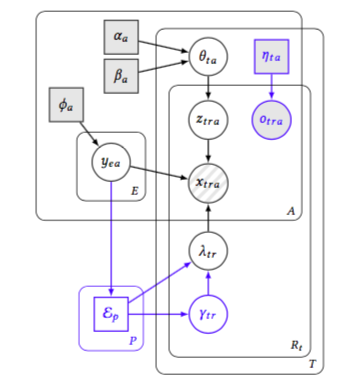
\includegraphics[scale=0.5]{figure/plate}
  \caption{
    Circular nodes denote random variables, square nodes denote 
    deterministic variables, (un)shaded nodes denote (un)observed
    variables, and arrows denote conditional dependence.
    %Squiggly line: selector connection (selects index for a co-connected matrix/vector variable).
    }
\label{default}
\end{center}
\end{figure}
}

\frame{
\frametitle{Remainder of the talk}

\begin{enumerate}
\item Present a simplified version of the model and tricks for performing inference.  
\item Why? To provide more intuition to users and practitioners. 
\item Present experiments/demos using the generalized model. 
%Our experiments and demos are given using the generalized model, and we will walk users through this. 
\end{enumerate}
\vspace*{1em}

A demo of the software will be presented at the end of the talk in Apache Spark. 
%is not publicly available at this time or software, however, if you are interested in this and providing feedback, please speak with me after the short course. 
}



\frame{
\frametitle{Overview of d-blink}

\begin{minipage}{0.47\textwidth}
\begin{enumerate}
\item Entity attributes
\begin{itemize}
\item Use the empirical distribution function
\item Assume attributes are independent
\end{itemize}
\item Links from entities to attributes
\item Record attributes 
\begin{itemize}
\item Hit and miss distortion prior
\item When distorted draw from attribute domain based on similarity to non-distorted value 
\end{itemize}
\end{enumerate}
\end{minipage}
\begin{minipage}{0.5\textwidth}
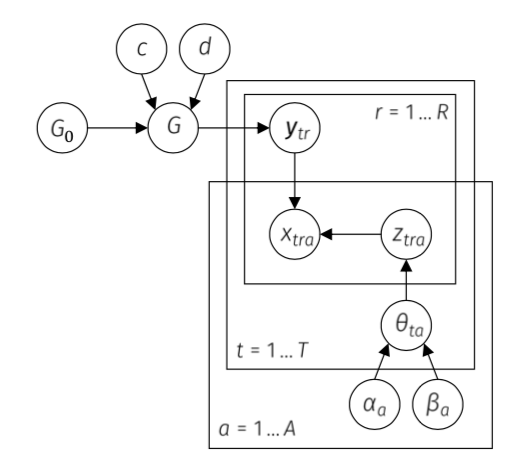
\includegraphics[width=\textwidth]{dblink/graphical-model-neil}
\end{minipage}


}




\frame{
\frametitle{Overview of d-blink}

\begin{minipage}{0.47\textwidth}
\begin{enumerate}
\item \textcolor{orange}{Entity attributes}
\begin{itemize}
\item \textcolor{orange}{Use the empirical distribution function}
\item \textcolor{orange}{Assume attributes are independent}
\end{itemize}
\item Links from entities to attributes
\item Record attributes 
\begin{itemize}
\item Hit and miss distortion prior
\item When distorted draw from attribute domain based on similarity to non-distorted value 
\end{itemize}
\end{enumerate}
\end{minipage}
\begin{minipage}{0.5\textwidth}
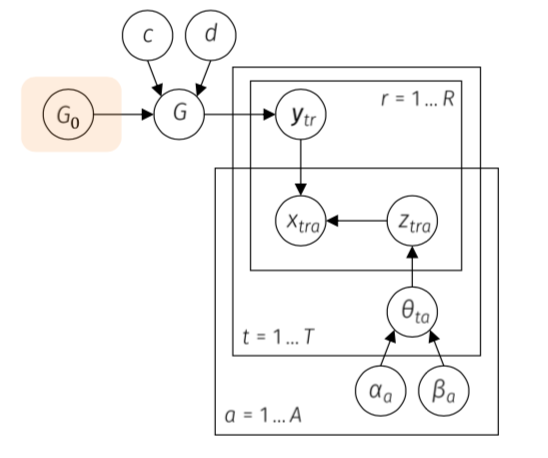
\includegraphics[width=\textwidth]{dblink/graphical-model-1}
\end{minipage}


}


\frame{
\frametitle{Overview of d-blink}

\begin{minipage}{0.47\textwidth}
\begin{enumerate}
\item Entity attributes
\begin{itemize}
\item Use the empirical distribution function
\item Assume attributes are independent
\end{itemize}
\item \textcolor{orange}{Links from entities to attributes}
\item Record attributes 
\begin{itemize}
\item Hit and miss distortion prior
\item When distorted draw from attribute domain based on similarity to non-distorted value 
\end{itemize}
\end{enumerate}
\end{minipage}
\begin{minipage}{0.5\textwidth}
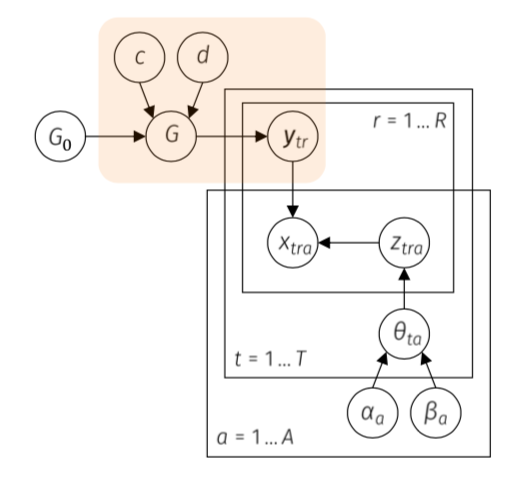
\includegraphics[width=\textwidth]{dblink/graphical-model-2}
\end{minipage}


}

\frame{
\frametitle{Overview of d-blink}

\begin{minipage}{0.47\textwidth}
\begin{enumerate}
\item Entity attributes
\begin{itemize}
\item Use the empirical distribution function
\item Assume attributes are independent
\end{itemize}
\item Links from entities to attributes
\item \textcolor{orange}{Record attributes}
\begin{itemize}
\item \textcolor{orange}{Hit and miss distortion prior}
\item \textcolor{orange}{When distorted draw from attribute domain based on similarity to non-distorted value}
\end{itemize}
\end{enumerate}
\end{minipage}
\begin{minipage}{0.5\textwidth}
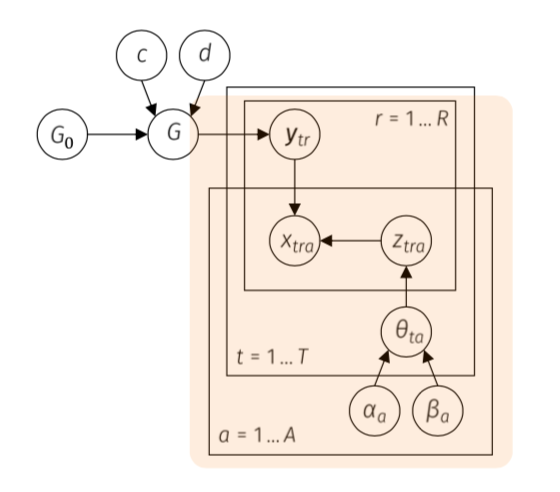
\includegraphics[width=\textwidth]{dblink/graphical-model-3}
\end{minipage}


}

\frame{
\frametitle{d-blink model}


\begin{figure}[htbp]
\begin{center}
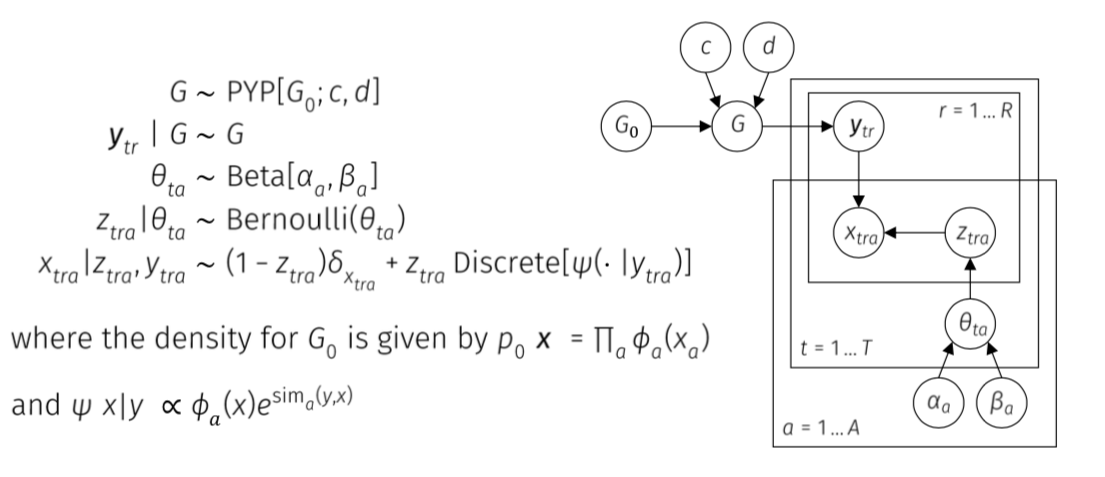
\includegraphics[width=\textwidth]{dblink/model}
%\caption{default}
%\label{default}
\end{center}
%\scriptsize{
%\begin{flushright}
%[Steorts, Hall, and Fienberg (2014), \emph{AIStats}.] \newline
%[Steorts, Hall, and Fienberg (2014), \emph{JASA}, In Revision], [Steorts (2014), Submitted.] 
%\end{flushright}
%}
\end{figure}


}

\frame{
\frametitle{Gibbs sampler}

\begin{minipage}{0.47\textwidth}
\begin{enumerate}
\item Reduce the problem to a sequence of low-dimensional simulations:
\begin{itemize}
\item Conditional distributions must be known and easy to sample from
\end{itemize}
\item Details for this model
\begin{itemize}
\item Partially-collapse the distortion indicators to improve mixing
\item Need to introduce auxiliary variables to update the hyper-priors
\end{itemize}
\end{enumerate}
\end{minipage}
\begin{minipage}{0.5\textwidth}
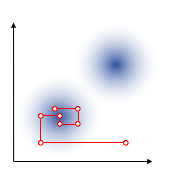
\includegraphics[width=\textwidth]{dblink/gibbs-sampler}
\end{minipage}

}

\frame{
\frametitle{Gibbs sampling tricks}

\begin{minipage}{0.47\textwidth}
Naive approach scales pooly:
\begin{enumerate}
\item Linkage structure update: O($\#$ entities $\times \#$ records)
\item Entity attribute update: O($\#$ entities $\times$ domain size)
\end{enumerate}
\end{minipage}
\begin{minipage}{0.5\textwidth}
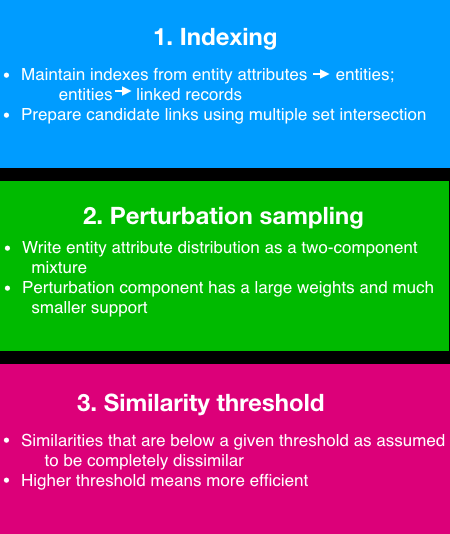
\includegraphics[width=\textwidth]{dblink/gs-tricks}
\end{minipage}




}



\frame{
\frametitle{Experiments}

\begin{itemize}
  \item \texttt{ABSEmployee}. A synthetic data set used 
  internally for linkage experiments by the ABS.
%  It simulates an employment census and two supplementary 
%  surveys. 
  \item \texttt{NCVR}. Two snapshots from the North Carolina 
  Voter Registration database taken two months 
  apart. 
%  The snapshots are filtered to include only those voters 
%  whose details changed over the two-month period.
%  We use the full name, age, gender and zip code attributes.
  \item \texttt{NLTCS}. A subset of the National Long-Term 
  Care Survey comprising the 
  1982, 1989 and 1994 waves.
  %\footnote{A subset must be used as race was 
  %subsampled in the other three years, making it unsuitable for ER.}
  % NM-1: Removing this footnote purely to fix the layout.
  % RS: Okay. 
%  We use the SEX, DOB, STATE and REGOFF attributes.
  \item \texttt{SHIW0810}. A subset from the Bank of Italy's 
  Survey on Household Income and Wealth
  comprising the 2008 and 2010 waves.
  %\footnote{Available at \url{http://github.com/[REDACTED]}} 
%    We use 8 attributes: IREG, SESSO, ANASC, STUDIO, PAR, 
%  STACIV, PERC and CFDIC.
  % NM-1: The SHIW data set we used is _different_ to the one 
  % that appears in the italy R package.
  % The version we used is based on the raw data from the 
  % Bank of Italy website, with a correction to the NORD 
  % variable (done using an R script that I wrote).
  % I guess we could make this available on GitHub...
  % RS-1: Thanks for clarifying. Would be helpful to put on Github since they are different and there could be confusion with the two different versions. 
  
  \item \texttt{RLdata10000}. A synthetic data set provided 
  with the \texttt{RecordLinkage} R 
  package. % because all attributes are missing.
  % NM-1: This is not true. There are "non-missing" values 
  % in fname_c2 and lname_c2 for RLdata10000 
  % (you might be thinking of RLdata500?).
  % RS-1: Yes. Thank you, NM! 
\end{itemize}

}


\frame{
\frametitle{Results}

The proposed method is applied to three real applications, with comparisons to standards in the literature. 


\tiny{
\newcolumntype{Y}{>{\centering\arraybackslash}X}
\begin{table}
	\centering
	\caption{Summary of the data sets used in the experiments. 
		Data sets marked with a `$\star$' are synthetic.}
	\begin{tabularx}{0.7\textwidth}{l *{3}{c} *{2}{Y}}
		\toprule
		Data set    & \# records ($M$) & \# files ($K$) & \# entities & \multicolumn{2}{c}{\# attributes ($L$)} \\
		\cmidrule{5-6} 
		 & & & & cat.\ & str.\ \\
		\midrule
		$\star$ \texttt{ABSEmployee} & 594,619 & 3 & 372,053 & 4 & 0 \\
		\texttt{NCVR}        & 448,134 & 2 & 296,433 & 3 & 3 \\
		\texttt{NLTCS}       &  57,077 & 3 &  34,945 & 6 & 0 \\
		\texttt{SHIW0810}    &  39,743 & 2 &  28,584 & 8 & 0 \\
		$\star$ \texttt{RLdata10000} &  10,000 & 1 &   9,000 & 2 & 3 \\
		\bottomrule
\end{tabularx}
\end{table}
}

}

\frame{



\scriptsize{
\begin{table}
	\centering
	\caption{Assessment of the pairwise linkage performance for dblink and FS method as our baseline. We note that FS is supervised and does not propagate the entity resolution error exactly compared to dblink. }
	\begin{tabular}{l l *{3}{c}}
		\toprule
		Data set    & Method & \multicolumn{3}{c}{Pairwise measure} \\
		\cmidrule(){3-5}
		 & & Precision & Recall & F1-score \\
		\midrule
		\multirow{2}{*}{\texttt{ABSEmployee}} 
		 & dblink                  & \textbf{0.9943} & \textbf{0.8867} & \textbf{0.9374} \\
		 & Fellegi-Sunter (100)  & {0.9964} & {0.9510} & {0.9736} \\
		 & Fellegi-Sunter (10)  & {0.4321} & {0.6034} & {0.9736} \\

		 
%		 & Near matching         & 0.0543 & \textbf{0.9970} & 0.1030 \\
%		 & Exact matching        & \textbf{0.9964} & 0.8849 & 0.9374 \\
		\midrule
		\multirow{2}{*}{\texttt{NCVR}}
		 & dblink                 & \textbf{0.9179} & \textbf{0.9654} & \textbf{0.9411} \\
		 & Fellegi-Sunter (100)  & 0.8989 & {0.9974} & {0.9456} \\
		 & Fellegi-Sunter (10)  & 0.8989 & {0.9974} & {0.9456} \\
%		 & Near matching         & 0.9899 & 0.7443 & 0.8497 \\
%		 & Exact matching        & \textbf{0.9925} & 0.0017 & 0.0034 \\
		\midrule
		\multirow{2}{*}{\texttt{NLTCS}}
		 & dblink                  & \textbf{0.8363} &  \textbf{0.9102} &  \textbf{0.8717} \\
		 & Fellegi-Sunter (100)  & 0.7969 & {0.9959} & {0.8853} \\
		  & Fellegi-Sunter (10)  & 0.1902 & {0.9999} & {0.3196} \\
%		 & Near matching         & 0.0385 & 0.9656 & 0.0740 \\
%		 & Exact matching        & \textbf{0.8451} & 0.9234 & 0.8825 \\ 
		\midrule
		\multirow{2}{*}{\texttt{SHIW0810}}
		 & dblink                  & \textbf{0.2529} & \textbf{0.5378} & \textbf{0.3440} \\
		 & Fellegi-Sunter (100)  & 0.1263 & {0.8480} & 0.2198 \\
		& Fellegi-Sunter (10)  & 0.0947 & {0.9244} & 0.1719 \\
%		 & Near matching         & 0.0043 & \textbf{0.9111} & 0.0086 \\
%		 & Exact matching        & 0.1263 & 0.7608 & 0.2166 \\ 
		\midrule
		\multirow{2}{*}{\texttt{RLdata10000}}
		 & dblink                  & \textbf{0.6310} & \textbf{0.9970} & \textbf{0.7729} \\
		 & Fellegi-Sunter (100)  & {0.9153} & {0.9940} & {0.9530} \\
		 & Fellegi-Sunter (10)  & 0.1706 & {1.0000} & 0.2915 \\
%		 & Near matching         & 0.9176 & 0.9690 & 0.9426 \\
%		 & Exact matching        & \textbf{1.0000} & 0.0080 & 0.0159 \\ 
		\bottomrule
	\end{tabular}
\end{table}
}



%\frame{
%
%\tiny{
%\begin{table}
%  \centering
%  \caption{Assessment  dblink and 
%    four baseline methods.
%    ``ARI'' stands for Adjusted Rand index and ``Err. \# clust.'' 
%    is the percentage error in the number of clusters.
%    %We cannot compute the cluster measures for Fellegi-Sunter and 
%    %Near Matching, since they do not guarantee transitivity of closure.
%    % RS-1: Could we add the estimates of N and the standard error as well 
%    % with a winner compared to the truth?
%    %
%    % NM-1: We could only do this for methods that ensure transitivity of 
%    % closure---i.e. blink and exact matching. I guess we could have another 
%    % grouped column called "Cluster measure" with sub columns: 
%    % "Adj. Rand index" and "relative error in # obs. entities".
%    % And for FS and near matching, the corresponding cells would have to be 
%    % "NA".
%    % RS-2: Yes, this is what I was thinking. 
%  }
%  \label{tbl:linkage-quality}
%  \begin{tabular}{l l *{5}{c}}
%    \toprule
%    Data set    & Method & \multicolumn{3}{c}{Pairwise measures} & \multicolumn{2}{c}{Cluster measures} \\
%    \cmidrule(lr){3-5} \cmidrule(lr){6-7}
%    & & Precision & Recall & F1-score & ARI & Err. \# clust.\ \\
%    \midrule
%    \multirow{5}{*}{\texttt{ABSEmployee}} 
%    & dblink             & 0.9763 & 0.8530 & \textbf{0.9105} & 0.9105 & \textbf{+1.667\%} \\
%    & Fellegi-Sunter (10)   & \textbf{0.9963} & 0.8346 & 0.9083 & --- & --- \\
%    & Fellegi-Sunter (100)  & \textbf{0.9963} & 0.8346 & 0.9083 & --- & --- \\
%    & Near Matching         & 0.0378 & \textbf{0.9930} & 0.0728 & --- & --- \\
%    & Exact Matching        & 0.9939 & 0.8346 & 0.9074 & 0.9074 & +9.661\% \\
%    \midrule
%    \multirow{5}{*}{\texttt{NCVR}}
%    & dblink\             & 0.9194 & \textbf{0.9634} & \textbf{0.9409} & \textbf{0.9409} & \textbf{--3.257\%}\\
%    & Fellegi-Sunter (10)   & 0.9868 & 0.7874 & 0.9083  & --- & ---\\
%    & Fellegi-Sunter (100)  & 0.9868 & 0.7874 & 0.9083 & --- & --- \\
%    & Near Matching         & 0.9899 & 0.7443 & 0.8497 & --- & --- \\
%    & Exact Matching        & \textbf{0.9925} & 0.0017 & 0.0034 & 0.0034 & +51.09\% \\
%    \midrule
%    \multirow{5}{*}{\texttt{NLTCS}}
%    & dblink             & 0.8360 & 0.9103 & 0.8716 & 0.8716 & --21.62\% \\
%    & Fellegi-Sunter (10)   & \textbf{0.9094} & 0.9087 & \textbf{0.9090} & --- & --- \\
%    & Fellegi-Sunter (100)  & \textbf{0.9094} & 0.9087 & \textbf{0.9090} & --- & --- \\
%    & Near Matching         & 0.0600 & \textbf{0.9563} & 0.1129 & --- & --- \\
%    & Exact Matching        & 0.8995 & 0.9087 & 0.9040 & 0.9040 & \textbf{+2.026\%} \\ 
%    \midrule
%    \multirow{5}{*}{\texttt{SHIW0810}}
%    & dblink           & \textbf{0.2517} & 0.5391 & \textbf{0.3432} & \textbf{0.3432} & --37.54\% \\
%    & Fellegi-Sunter (10)   & 0.0028 & 0.9050 & 0.0056 & --- & --- \\
%    & Fellegi-Sunter (100)  & 0.0025 & \textbf{0.9161} & 0.0050 & --- & --- \\
%    & Near Matching         & 0.0043 & 0.9111 & 0.0086 & --- & --- \\
%    & Exact Matching        & 0.1263 & 0.7608 & 0.2166 & 0.2166 & \textbf{--37.40\%} \\ 
%    \midrule
%    \multirow{5}{*}{\texttt{RLdata10000}}
%    & dblink            & 0.6302 & \textbf{0.9970} & 0.7723 & \textbf{0.7723} & 
%    \textbf{--10.95\%} \\
%    & Fellegi-Sunter (10)   & 0.9957 & 0.6174 & 0.7622 & --- & --- \\
%    & Fellegi-Sunter (100)  & 0.9364 & 0.8734 & 0.9038 & --- & --- \\
%    & Near Matching         & 0.9176 & 0.9690 & \textbf{0.9426} & --- & --- \\
%    & Exact Matching        & \textbf{1.0000} & 0.0080 & 0.0159 & 0.0159 & +11.02\% \\ 
%    \bottomrule
%  \end{tabular}
%\end{table}
%}




}

\frame{
\frametitle{Error in number of observed entities}


%Figure~\ref{fig:error-num-ents} displays error in posterior/prior estimates
%for the number of observed entities for dblink.

\begin{figure}[h!]
  \centering
  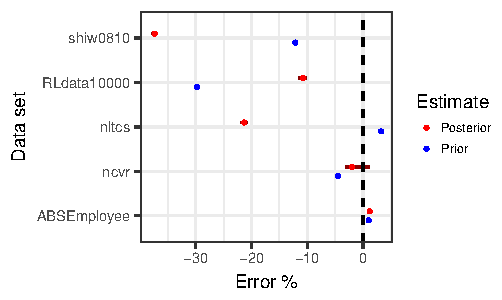
\includegraphics[width=0.8\textwidth]{figure/posterior-bias-plot.pdf}
  \caption{Error in the posterior and prior estimates for the 
    number of observed entities for dblink.
    The results show that the posterior estimate is very sharp 
    and typically underestimates the true number.
  }
  \label{fig:error-num-ents}
\end{figure}
}

%\frame{
%\frametitle{Posterior Bias Plot}
%
%\begin{figure}[htbp]
%\begin{center}
%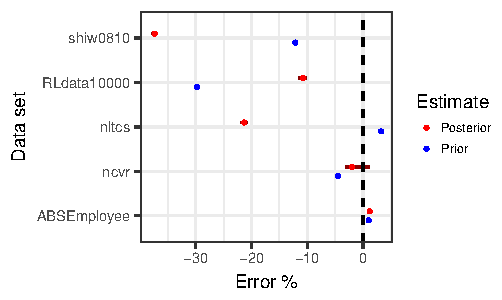
\includegraphics[scale=1]{figure/posterior-bias-plot}
%\caption{Error in the posterior and prior estimates for the number of observed entities for d-blink. The results show that the posterior estimate is very sharp and typically underestimates the true number, which is consistent with \textbf{RCS}, Hall, Fienberg (2016). }
%\label{default}
%\end{center}
%\end{figure}
%
%
%}

\frame{
\frametitle{Super-linear speed-up}
\begin{figure}
  \centering
  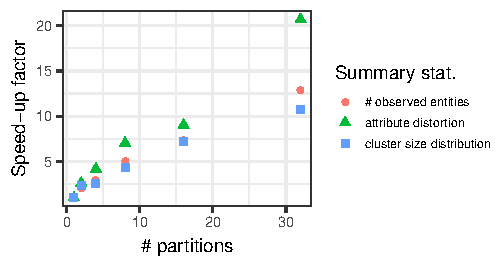
\includegraphics[width=0.6\textwidth]{figure/ess-plot-test-num-partitions-speed-up.pdf}
  \caption{Efficiency of d-blink as a function of partition size P and summary statistic of interest. The speed-up measures the ESS rate relative to the ESS rate for P = 1 (no partitioning) for the NLTCS data set.}
%  \caption{Real time speed-up with respect to the elapsed time for 
%    1~partition.
%    The benchmark was to reach an effective sample size (ESS) of 100 on 
%    the \texttt{NLTCS} data set.
%    Note that the speed-up varies depending on the summary statistic 
%    used to calculate the ESS.
%    Most points lie above the black line, indicating a super-linear 
%    speed-up.}
  \label{figure/speed-up-vs-num-partitions}
\end{figure}
}




%\frame{
%\begin{figure}
%  \centering
%  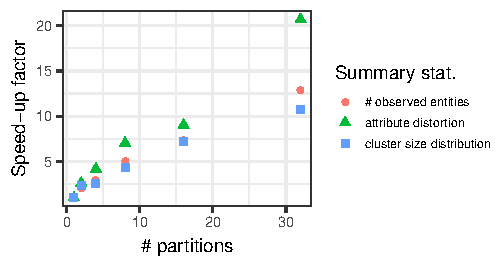
\includegraphics[width=0.8\textwidth]{figure/ess-plot-test-num-partitions-speed-up.pdf}
%  \caption{Real time speed-up with respect to the elapsed time for 
%    1~partition.
%    The benchmark was to reach an effective sample size (ESS) of 100 on 
%    the \texttt{NLTCS} data set.
%    Note that the speed-up varies depending on the summary statistic 
%    used to calculate the ESS.
%    Most points lie above the black line, indicating a super-linear 
%    speed-up.}
%  \label{figure/speed-up-vs-num-partitions}
%\end{figure}
%}

\frame{
\frametitle{Demo of dblink}

\begin{enumerate}

\item I will now give a quick demo of the dblink in Apache Spark on the \texttt{RLdata500} data set. 

\item dblink once available will be public at \url{https://github.com/ngmarchant/dblink}. 

\item The guide for running the package can be found at \url{https://github.com/ngmarchant/dblink/blob/master/docs/guide.md}


\end{enumerate}

}



\frame{
\frametitle{Takeaways}

\begin{enumerate}
\item Our methods are very scalable and the first of our knowledge for Bayesian entity resolution. 
\item The Bayesian approach allows for a full posterior and exact error propagation into downstream tasks (like regression). 
\item Our methods perform as well if not better than state-of-the-art methods in practice. 
\item With more computing resources, we can scale to larger data sets, which we're currently investigating. 
\end{enumerate}

}




\frame{
\frametitle{Thank you!}

\center
Questions? \\
beka@stat.duke.edu\\
resteorts.github.io \\

\vspace*{1em}

Thank you to the National Science Foundation for NSF CAREER Microclustering and NSF Big Data Privacy. The views in this talk are of the authors alone and not of the funding organization. \\



%\vspace*{1em}
%Copas and Hilton (1990)\\
%Larsen and Lahiri (2005) \\ 
%Tancredi and Liseo (2011)\\ 
%Kim and Chambers (2012) \\ 
%Gutman, Afendulis, Zaslavsky (2013) \\ 
%\textbf{RCS}, Hall, Fienberg (2016), JASA. \\
%Betancourt, Zanella, Miller, Wallach,  \textbf{RCS}, NIPS (2016). 
%Chen, Shrivastava, \textbf{RCS} (2018), AOAS \\
%Marchant, Kaplan, Rubenstein, and \textbf{RCS} (2018), To be Submitted. \\
%Kaplan, Betancourt, \textbf{RCS} (2018), Submitted. \\






}







\end{document}